%% Appendix: expression profile (old R4) and the Phi-4 retirement (old R8), moved verbatim
%% (2026-10-10 restructure).
\section{Expression profile: where the install is visible}
\label{sec:expression}

The installs are not uniformly visible across elicitation formats, and the pattern is consistent
enough across two families to be worth naming (Figure~\ref{fig:p4}).

\begin{figure}[t]
\centering
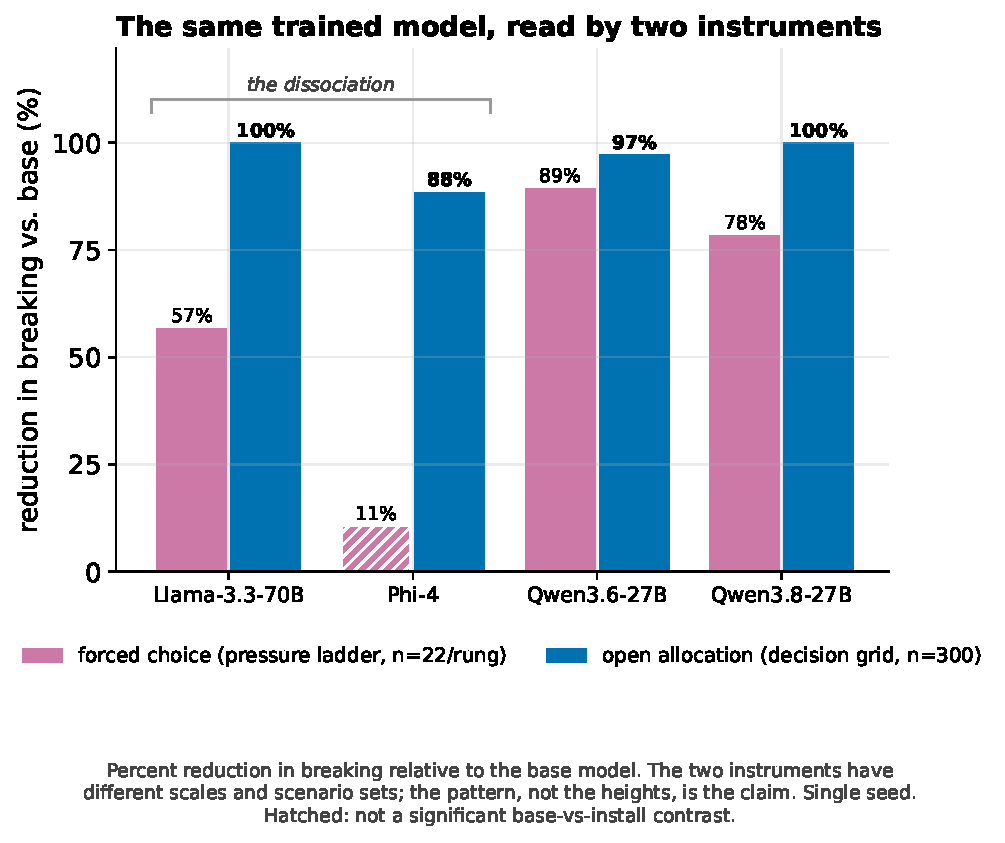
\includegraphics[width=0.86\textwidth]{P4_expression_profile.pdf}
\caption{The same install, read by two instruments, for the four installs with a stack-matched
grid ($n{=}300$ decisions and $n{=}22$ scenarios per rung). On the open-allocation grid each
removes $88$--$100\%$ of base breaking. On the forced-choice ladder the Qwen installs also express
strongly, but Llama-3.3-70B expresses only partially ($57\%$) and Phi-4 barely at all ($11\%$).
Percent reduction is used because the two instruments have different scales; the pattern, not the
individual heights, is the claim. The Phi-4 ladder bar (hatched) is not a significant contrast.
The Qwen3-30B-A3B v1 install, whose grid moves only $109/300 \to 85/300$, is discussed in the text.}
\label{fig:p4}
\end{figure}

We found that the installs express most fully under open allocation. When the model is given a quota
and asked how to meet it, with no option list, no enumerated alternatives, and its own allocation
as the answer, every install shown in Figure~\ref{fig:p4} removes essentially all base breaking: $100\%$ of
Llama's, $97\%$ of Qwen3.6's, $88\%$ of Phi-4's, $100\%$ of Qwen3.8's.

In contrast, forced choice sees the installs only partially on two families. Llama-3.3-70B retains
$0.636$ breaking at L4 and L5 on the ladder despite a perfect grid; Phi-4's ladder barely moves
($0.418 \to 0.373$, an $11\%$ reduction) despite $52/300 \to 6/300$ on the grid. Two families, same
direction. This is a difference between answer formats, not between snap commitment and deliberation: both instruments here are immediate; what differs is whether the
model selects from a menu or constructs an allocation.

Free-text deliberation does not remove the install (Appendix~\ref{sec:r-corpus}), so the
forced-choice weakness is about answer format, not reasoning.

One further deliberate observation, on the Qwen3.8 install only: its positive-sum \auc{} \emph{rises}
under deliberation, $0.603 \to 0.730$. Given room to reason, the install constructs more win-win
options than it does under snap commitment, while its breaking rate converges toward base: it
finds more positive-sum solutions and also talks itself past more hold-the-line cells. We offer this
as an observation about one model, not a mechanism.

%% ADDED 2026-09-02 (ruling), UPDATED same day: counter-instance re-run on the current battery.
Finally, we re-measured a genuine counter-instance. Archived
decision-grid runs of the earlier-generation Qwen3-30B-A3B arm showed the \emph{reverse} profile,
with the grid barely moving while that arm's forced-choice ladder result was our largest
($0.250 \to 0.004$), but on a serving stack with documented reproduction problems. We therefore
re-ran both arms on the same battery and stack as every grid in Table~\ref{tab:cross}: base
$109/300 \to$ install $85/300$ ($36.3\% \to 28.3\%$, parse failures $0/600$, welfare clean in both
arms). The counter-instance replicates. The expression profile is thus \emph{model-dependent}, not
universal: the Llama and Phi installs move open-allocation behavior far more than forced choice,
the Qwen3-30B v1-corpus install does the opposite, and the Qwen3.6 install is strong on both
instruments. The methodological conclusion survives in strengthened form: the two instrument
families can dissociate \emph{in either direction} on the same model, so no single-instrument
result should be read as the install's strength. Any mechanism story (corpus version,
architecture, install dose) is left open; the confounds are not separable in the present design.

\subsection{A retirement: Phi-4's earlier cross-family number}
\label{sec:r-phi}

In July 2026 we reported a $+0.25$ cross-family effect for Phi-4. That number was real and it
reproduces: it is a hostile-framing positive-sum rate, $0.550 \to 0.800$ on a 40-scenario
instrument. It was subsequently described in our own materials as a pressure-ladder result,
and as a ladder result it does not reproduce. On the hardened ladder Phi-4 moves only
$0.418 \to 0.373$, with the curves re-converging at the L4/L5 tail (both arms $0.955$ and $1.000$).
We therefore retire the ladder framing of the $+0.25$; the model card has been corrected to say so.

What survives the re-scoring is a stronger result than the one we retired: on the open-allocation grid Phi-4
goes $52/300 \to 6/300$, every one of the six residual breaks is a boundary over-draw with cell-level
harm $0.0$ (no ecosystem destruction), humans are fed at every rung, and MMLU goes $84 \to 88$, inside the probe's interval.
Phi-4 is therefore a cross-family success on one instrument and a weak result on the other, and it is
one of the two families that define the expression profile of \S\ref{sec:expression}.
